\documentclass{article}
%\documentclass{amsart}
 


%%%%%%%%%%%%%%%%%%%%%%%%%%%%%%%%%%%%%%%%%%%%%%%%%%%%%%%%%%%%%%%%%%%%%%%%%%%%%%%
% language support
\usepackage{xeCJK}

% xcolor
\usepackage[dvipsnames]{xcolor}

% indentfirst
%% 添加首行缩进,两个字符,用于中文文档
%% 用于英文文档时注释以下两行
\usepackage{indentfirst}
\setlength{\parindent}{2em}

% math
\usepackage{amsfonts,amsmath,amssymb,amsthm}
\usepackage{bm}
\usepackage{mathtools}
%% define new
\newtheorem{definition}{Definition}[section]
\newtheorem{axiom}{Axiom}[section]
\newtheorem{theorem}{Theorem}[section]
\newtheorem{corollary}{Corollary}[theorem]
\newtheorem{lemma}[theorem]{Lemma}
\newtheorem*{remark}{Remark}
\newtheorem*{exercise}{Exercise}

% hyperref
\usepackage{hyperref}
\hypersetup{
	colorlinks=true,
	linkcolor=blue,
	pdftitle={SELinux},
}

% acronym
\usepackage[acronym]{glossaries-extra}
\setabbreviationstyle[acronym]{long-short}
\makeglossaries
\newacronym{selinux}{SELinux}{Security-Enhanced Linux}
\newacronym{dac}{DAC}{Dictionary Access Control}
\newacronym{mac}{MAC}{Mandatory Access Control}
\newacronym{dbms}{DBMS}{Database Management system}
% tcolorbox
\usepackage{tcolorbox}

% geometry
%% it's useful to adjust page margins and line spacing.
% \usepackage[left=2cm, right=2cm, top=1.54cm, bottom=1cm]{geometry}
\usepackage[margin=2.5cm]{geometry}

% fancyhdr
%% fancyhdr 需要放在 geometry 后面
\usepackage{fancyhdr}
\pagestyle{fancy}
\fancyhead[R]{\leftmark} % 设置右页眉为章节标题


% setspace
%% a simple way of changing line spacing
%% e.g. for 1.5x line spacing
% \usepackage[onehalfspacing]{setspace}
%% [doublespacing] for 2x line spacing

% siunitx
\usepackage{siunitx}

% graphicx
%% include the graphics
%% e.g. scale the image to 80% of the text width
% \includegraphics[width=0.8\textwidth]{figure.eps}
%% e.g. fix the hight and width of a figure
%% [width=2cm, height=5cm]
%% e.g. rotate 90 degrees
%% [angle=90]
%% set the default path
% \graphicspath{{./figures}{./additionalFigures}}

% biblatex
% \usepackage{biblatex}

% lineno
%% 每行数字序列
% \usepackage{lineno}
% \linenumbers


\newcommand{\bsl}{\texttt{\symbol{92}}}



\title{多组热管散热器空气源热泵的实验研究}
\author{Shuxue~Xu, Jianhui~Niu, Guoyuan~Ma}

\begin{document}
\maketitle

\begin{abstract}
作为一种清洁、可持续电气化供暖技术,空气源热泵 (ASHP) 已在中国家庭中得到广泛应用。然而,常用的水循环系统存在效率低、结构复杂、易冻裂、电能消耗高等问题。本文提出了一种新型多组热管散热空气源热泵 (ASHPMP)。在 ASHPMP 系统中,冷凝器和热管耦合在一起,形成一种新型的热辐射终端,被命名为热管散热器,由压缩机驱动的多个终端为多个房间提供热量。开发 ASHPMP 系统的实验装置,并在住宅楼中进行了实验,热泵使用 R410A,热管使用 R134a。分析结霜与除霜条件下温度、热泵和热管压力对 ASHPMP 供热性能的影响。结果表明,新系统可在室外温度为$\qty{-12.7}{\degreeCelsius} $至$\qty{6.5}{\degreeCelsius} $的条件下稳定运行. 当室内温度设定为$\qty{20}{\degreeCelsius} $, 室外温度为$\qty{-12.7}{\degreeCelsius} $时, 制热性能系数(制热 COP)可达 3.15, 室外温度为$\qty{6.5}{\degreeCelsius} $时, 制热性能系数为 6.73.

\noindent \textbf{关键字:} 空气源热泵; 热管散热器; 供热性能; 应用研究
\end{abstract}

\section{导言}
研究表明,燃烧导致的的碳排放呈上升趋势。随着经济的快速发展,煤碳消耗量不断增加,环境污染日益严重。在中国京津冀地区, 2014 年燃煤造成的 PM2.5 浓度占年均值的 28.5\%。最近几年,中国大多数城市的空气质量已引起人们的关注,持续减少燃煤消耗是唯一的办法,尤其是在农村地区冬季取暖的建筑能耗居高不下的情况下。为减少 \ce{CO2} 排放和 PM2.5,中国实施了一系列政策和措施,如“煤改电”计划,重点是用电采暖设备替代化石燃料。

热泵是一种具有不同用途的高效换热设备,可利用各种能源工作。文献提出了一种利用浴室排水余热的新型热泵系统。文献将实验室的热泵装置改装成了冰箱,并使用对使用 R407C 制冷剂的新系统性能进行了研究。近年来,空气源热泵 (ASHP) 已经在中国北方地区,尤其是家电领域发挥着重要的作用。对于 ASHP 供热系统,散热器和空调 (AC) 是常用的供热终端,在中国的“京津冀”地区,90\% 以上的居民选择了热辐射终端。水流经室外机的冷凝器,从约$\qty{40}{\degreeCelsius}$加热到$\qty{60}{\degreeCelsius}$,然后在水泵的驱动下流入散热器,加热室内空气。

但也发现了一些问题,如效率低、结构复杂、更容易冻结和爆裂以及电能消耗高。为了避免二次换热,简化系统结构,直接将冷凝末端与 AHSP 相结合,许多研究都guan关注空调的室内热舒适性。事实上,空调的热不适感稍强,如强烈的穿堂风和室内噪音。作为另一种直接冷凝式采暖终端,AHSP 系统的制冷剂直接加热地板,许多研究都集中在直接地板辐射采暖的传热过程上。

作为一种高效的热交换器,热管被广泛应用于核反应堆冷却、电子设备 CPU 冷却,建筑物冷却、太阳能利用等。利用热管集热器/蒸发器作为蒸汽压缩热泵的另一种热源,构建了实验装置,结果表明机组的平均热容量和制热 COP 可分别提高 27.61\% 和 27.85\%。在冷凝器中插入热管以改善空调冷凝测的散热性能,实验结果表明能效比比传统空调高出 3.11\%。热管也可用于地源热泵系统,热管是收集低品味地热的关键部件。

在我们之前的研究中,提出了以热管作为散热器的 ASHP 系统,压缩机驱动热管向室内释放热量。实验研究了热管内部的传热过程、工作流体类型和充注量对系统性能的影响和系统工作性能随工况的变化等。文献验证了热管在空气源热泵中应用的可行性:
\begin{itemize}
    \item 热管表面的温度均匀性非常好,表面平均温度与热泵leng冷凝温度之间的差异非常校,仅为$\qty{1.5}{\degreeCelsius}$。
    \item 在室外温度为 -$\qty{15}{\degreeCelsius}$,室外温度为$\qty{22}{\degreeCelsius}$的情况下,新型 ASHP 系统的制热 COP 可达 2.55。
\end{itemize}

然而,这些研究只提出了但热管散热器系统的模式和原理,系统性能也是在实验室中研究的。对于谁环热泵系统来说,热水是通过水泵的驱动输送到多个房间的采暖末端。为了满足实际建筑的供暖需求,还需要将热泵系统做成多端型。当末端数量增加时,热管温度均匀性、系统稳定性、能效等方面的考虑就显得尤为重要。特别是在除霜工况下运行时,除霜效果、热管表面温度的下降值对其实际应用至关重要。

本文提出了一种带有多组热管散热器 (ASHPMP) 的空气源热泵系统。为了便于安装和将室内和室外机连接,多根热管的末端被串联起来。开发了一种实验方法,并在环境控制室进行了测试。压力、温度和其他参数
在实际供暖建筑和实际气象条件下对热泵和热管的压力、温度和其他参数进行了实验研究。在实际供暖建筑和实际气象条件下,对热泵和热管的压力、温度和参数进行了实验研究。还探讨了霜冻/结霜条件下系统供热性能的变化。还探讨了霜冻/结霜条件下系统供热性能的变化。


\section{ASHPMP 系统}
如图~\ref{F:1} 所示, ASHPMP 系统由压缩机、热管散热器、节流阀、蒸发器和管道组成。热管散热器、节流阀、蒸发器和管道组成。制冷剂从压缩机流出,进入 8 组冷凝器,这些冷凝器与热管共同构成热管散热器。热管散热器(HPR)。
每台设备都向室内释放热能、从而提高室内空气温度。

ASHPMP 系统的主要优点如下:
\begin{itemize}
    \item HPR 全部串联,安装和维护都很方便。
    \item 没有水箱、水泵和水管,不存在结霜风险。HPR 可以将热量迅速传递到室内,从而带来更加舒适惬意的供暖体验。
\end{itemize}

图~\ref{F:2} 显示了 HPR 的详细结构。如图~\ref{F:2a} 所示, HPR 由三大部分组成: 上收集管、下收集管和带散热片的热管。在下收集管中,如图~\ref{F:2b} 所示,由一个制冷剂入口管和出口管、一个压力表和一个制冷剂充注管,充注管作为维修阀门,用于抽真空和添加工作介质。冷凝管束插入其中。

为了降低成本,使用铝来制作 HPR。热管程度为 \qty{1.04}{m}, 高度为 \qty{0.8}{m},直径为 \qty{0.028}{m}。尺寸参数见图~\ref{F:3a},热管照片见图~\ref{F:3b}。

\begin{figure}[htbp]
	\centering
	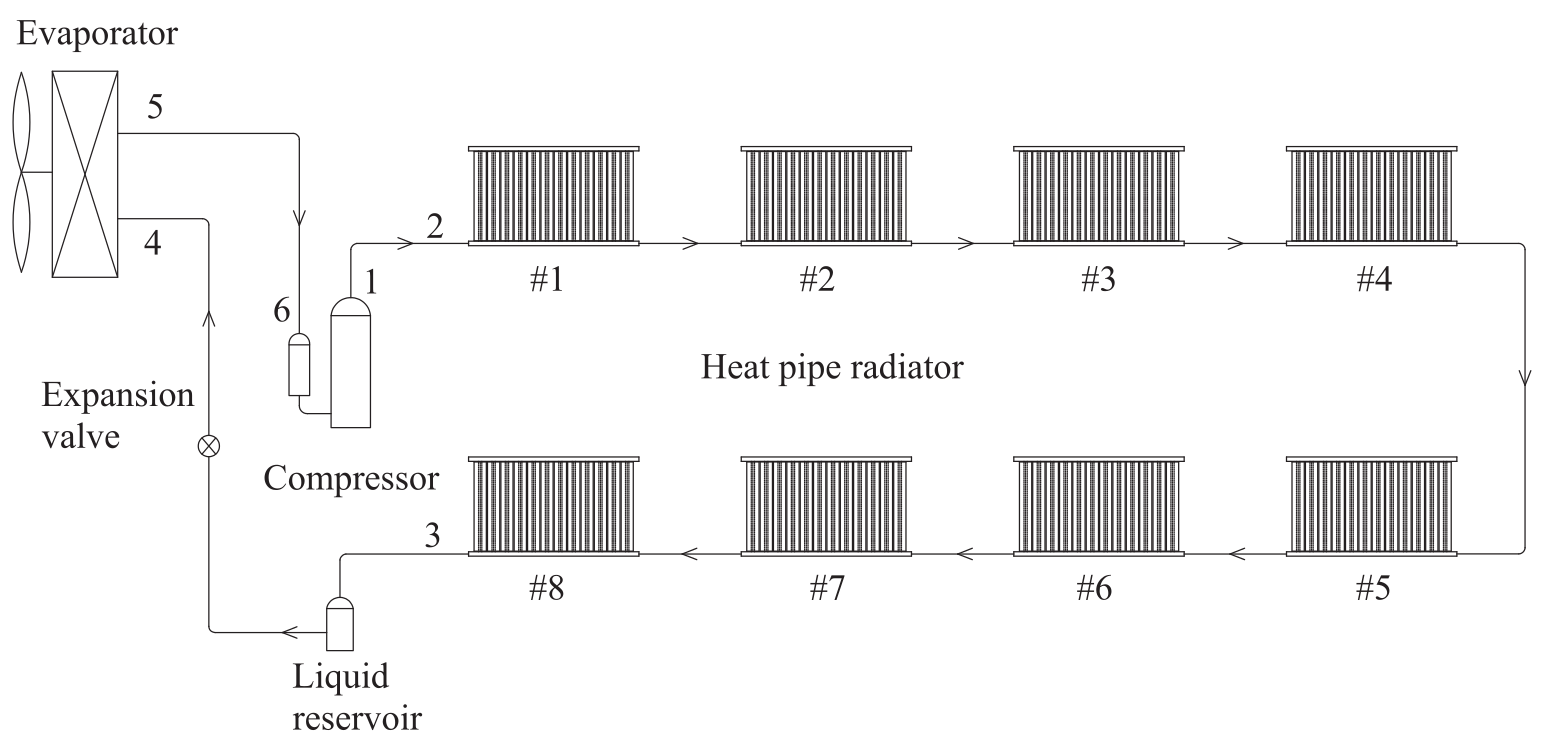
\includegraphics[width=0.7\textwidth]{picture/picture_1}
	\caption{ASHPMP 系统}
	\label{F:1}
\end{figure}

\begin{figure}[htbp]
\centering  %图片全局居中
\subfigure[HPR 结构参数]{
\label{F:2a}
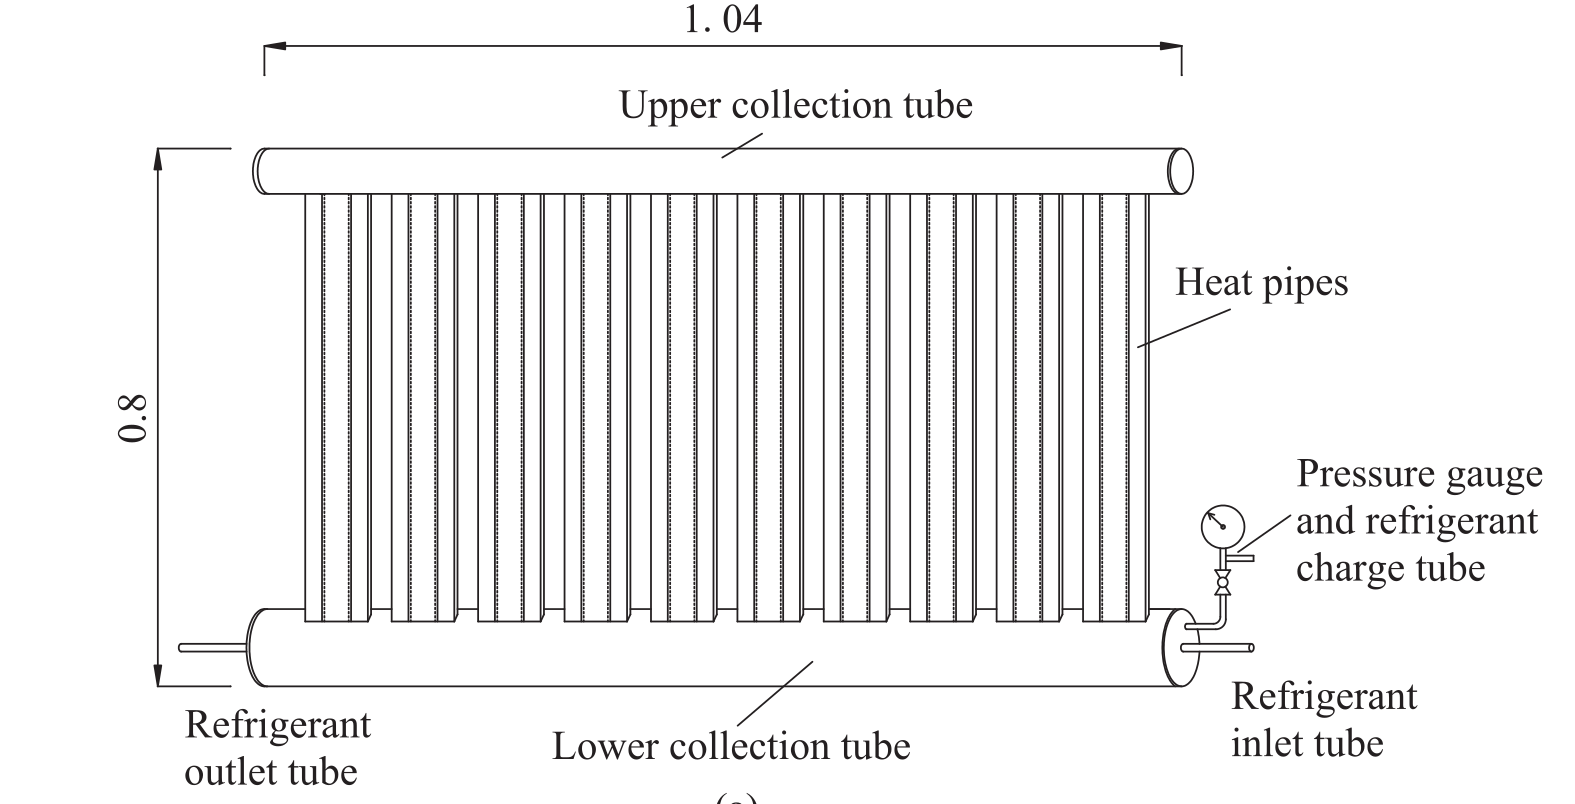
\includegraphics[width=0.7\textwidth]{picture/picture_2_a}}

\subfigure[下收集管的结构]{
\label{F:2b}
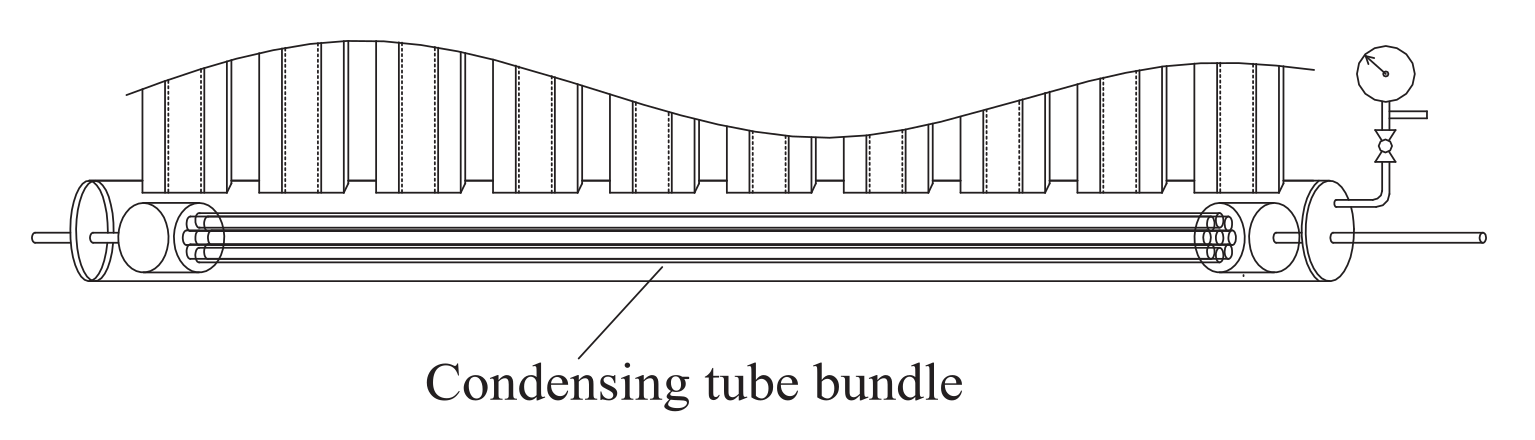
\includegraphics[width=0.7\textwidth]{picture/picture_2_b}}
\caption{HPR 和 冷凝器结构}
\label{F:2}
\end{figure}

\section{分析模型}
热泵冷凝器的热量通过强制对流传递给底部的热管制冷剂,然后通过液体和蒸汽空间传递给整个热管主体。最后,热量通过热管外表面的自然对流和辐射释放到室内空间中,
\begin{equation}\label{E:1}
	A = \frac{Q'_{r}}{h_c (t_f - T_i)} 
\end{equation}
其中,$Q'_r$ 为每根热管的散热量 $(\unit{\kW})$;$A$ 为表面积 $(\unit{\m^2)}$;$h_c$ 为复合传热系数 $(\unit{\kW/(\m^2\K)} )$;$t_f$ 是表面温度 $(\unit{\degreeCelsius})$;$T_i$ 是室温 $(\unit{\degreeCelsius})$。

冷凝管束中的单根管子的长度计算公式为:
\begin{equation}\label{E:2}
	l = 1000 Q'_r \frac{\ln (d_o/d_i)}{2 \pi n \lambda \Delta t} 
\end{equation}
其中,$\Delta t$ 为铜管内外表面温差$(\unit{\degreeCelsius})$; $d_o$为铜管外径$(\unit{\m})$, $\lambda$为铜管导热系数 $(\unit{\W/(\m\K)})$; $l$ 为铜管长度 $(\unit{\m})$; $n$ 为铜管数量。

管壁两侧的传热温差已知,传热面积可根据公式~\ref{E:1} 已知管壁两侧的传热温差,则传热面积可根据公式~\ref{E:2}。如图~\ref{F:4a} 所示,在每根热管的下部收集管中插入 9 根直径为$\qty{0.008}{\m} $的铜管。下收集管的直径为$\qty{0.04}{\m} $,厚度为$\qty{0.003}{\m}$。如图~\ref{F:4a} 所示。冷凝器与图~\ref{F:4b} 显示了与 HPR 相结合的冷凝器的照片。表~\ref{T:1} 概述了 HPR 的主要结构尺寸。

\begin{figure}[h]
\centering  %图片全局居中
\subfigure[热管尺寸参数]{
\label{F:3a}
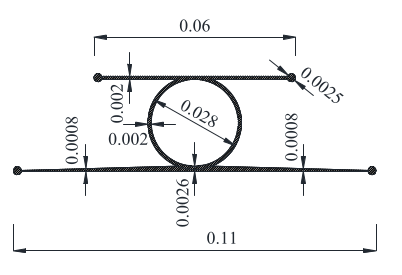
\includegraphics[width=0.3\textwidth]{picture/picture_3_a}}
\subfigure[热管照片]{
\label{F:3b}
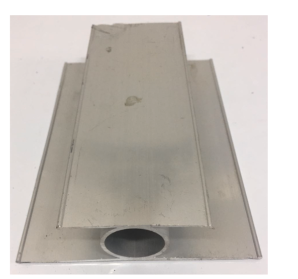
\includegraphics[width=0.3\textwidth]{picture/picture_3_b}}
\caption{热管尺寸与照片}
\label{F:3}
\end{figure}

\begin{figure}[h]
\centering  %图片全局居中
\subfigure[HPR 和 冷凝器的结构尺寸]{
\label{F:4a}
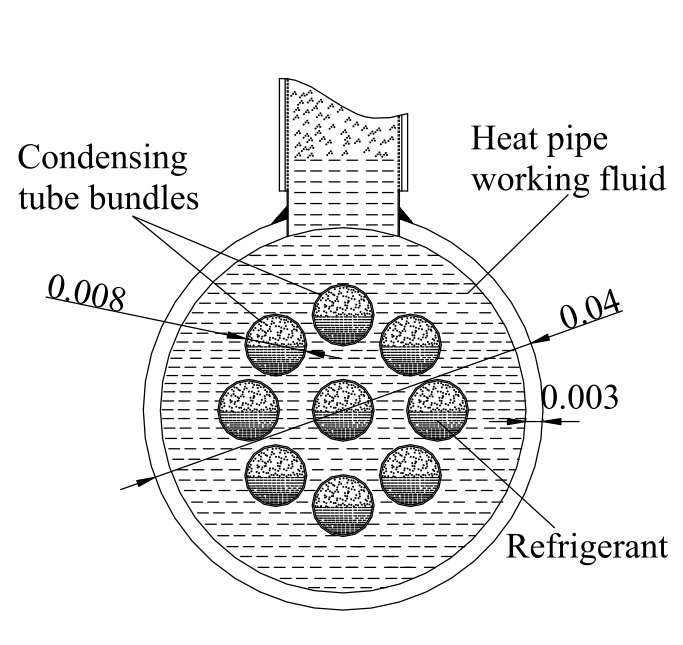
\includegraphics[width=0.3\textwidth]{picture/picture_4_a}}
\subfigure[配有 HPR 的冷凝器照片]{
\label{F:4b}
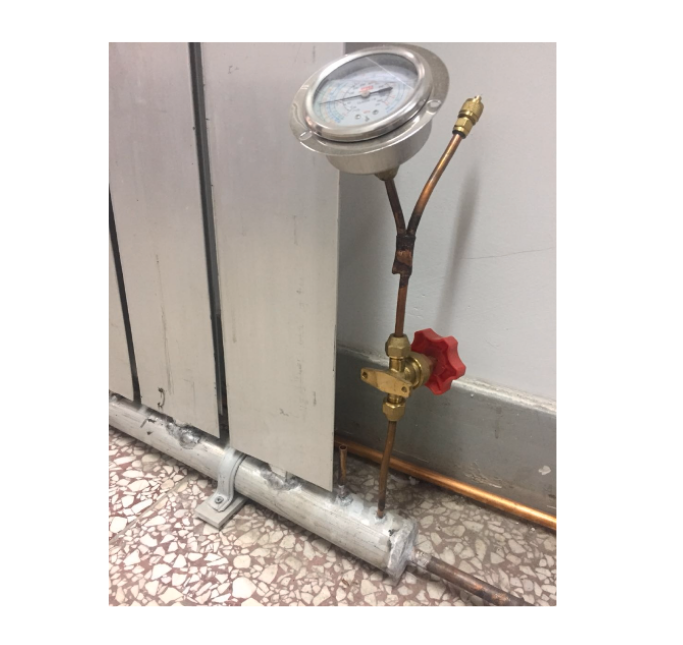
\includegraphics[width=0.3\textwidth]{picture/picture_4_b}}
\caption{HPR 与冷凝器的结构尺寸与照片}
\label{F:4}
\end{figure}

\begin{table}[ht]
\centering
\caption{主要尺寸结构}
\begin{tabular}{@{}lllllll@{}}
\toprule
宽度   & 高度  & 行号 & 尺寸    &       & 厚度    &       \\ \midrule
\qty{1.04}{\m} & \qty{0.8}{\m} & \qty{10}{\m} & 上下冷凝管 & 热管    & 上下冷凝管 & 热管    \\
     &     &    & \qty{0.04}{\m}   & \qty{0.028}{\m} & \qty{0.003}{\m} & \qty{0.002}{\m}  \\ \bottomrule
\end{tabular}
\label{T:1}
\end{table}

\section{实验设备}
新设备在中国北京进行了测试。如图~\ref{F:5} 所示试验室面积约为$\qty{25}{\m^2} $。压缩机排出的高温高压压缩机排出的高温高压蒸汽进入室内的 HPRs,再将热量传入室内。进而将热量传递到室内。热泵工作流体的热量工作流体的热量通过 HPR 散失。起初,制冷剂的状态可能保持不变,例如在 HPR \#1 中。在 HPR \#1 之后、温度降低的热泵制冷剂进入HPR \#2,继续通过 HPR 散热。此时,如果此时,如果第二台室内机的面积足够大,制冷剂将变成两相,并进入 HPR \#2。变成两相,进入 HPR \#3。同样,进入 \#4、\#5,直到最后一组。依次进入最后一组。当制冷剂从最后一个室内机流出时、工作介质是典型的过冷液体。

热管工作流体为 R134a。主要参数如每块热管的压力、室内外温度、空气侧进出口温度、室内室温等、室内室外温度、空气侧进出口温度、室内室温等主要参数。测量。为了研究系统中的压力分布,一定数量的压力传感器被安装在每个 HPRs 中,如图~\ref{F:5} 所示。

图~\ref{F:6} 展示了 ASHPMP 系统的照片,表~\ref{T:2} 列出了实验系统的规格。

压缩机的额定功率为$\qty{21}{\kW} $,工作流体为 R410A,由直流变频电机驱动。电机驱动,其频率在$\qty{0}{\hertz}$~\textasciitilde~$\qty{120}{\hertz} $之间变化。温度传感器设置在液态制冷剂管上,即膨胀阀之前的位置。当压缩机运行时,其转速由该温度点的设定值控制。当前温度低于设定温度时,压缩机转速会增加,当前温度低于设定温度时,压缩机转速会降低。当当前温度接近设定温度时,压缩机转速会降低。在一定的逻辑下,压缩机的速度根据当前温度和设定温度之间的差值来调节压缩机的转速。最后,最终控制温度温度波动范围很小。

压力传感器(不确定度 $\pm 5\%$)被用于测量热泵和热管的制冷剂压力。Pt100 温度传感器(不确定度 $\pm 5\%$)被用来测量空气和制冷剂温度。空气和制冷剂温度。液体管路中有一个质量流量计液体管路中装有质量流量计,可直接获得制冷剂的流量质量。不确定度 $\pm 5\%$ 的功率计用于监测压缩机的输入功率。压缩机的输入功率。加热能力Q $\unit{\kW} $和制热 COP 的不确定性可通过以下公式计算得出。仪器仪器和传播的不确定性总结如表~\ref{T:3}。

\begin{equation}\label{E:3}
	COP = \frac{Q}{W'} = \frac{m'(h_2 - h_3)}{W'} = f'(m',p_2,t_2,p_3,t_3,W')
\end{equation}

$m'$是制冷剂的质量流量$\unit{\kg/\s} $, $p_2, p_3$是制冷剂在图~\ref{F:5} 点 2 和 3 的压力$\unit{\MPa} $;$t_2, t_3$图~\ref{F:5} 点2 和 3 的制冷剂温度$\unit{\degreeCelsius} $; $h_2, h_3$是图~\ref{F:5} 点 2 和 3的焓$\unit{\kJ/\kg} $; $W'$是功率输入$\unit{\kW} $。

\begin{equation}\label{E:4}
	u_Q = \sqrt{(\frac{\partial f}{\partial m'} u_{m'})^2 + (\frac{\partial f}{\partial t_2} u_{t2})^2 + (\frac{\partial f}{\partial t_3} u_{t3} )^2+ (\frac{\partial f}{\partial p_2} u_{p2})^2 + (\frac{\partial f}{\partial t_2} u_{p3} )^2}
\end{equation}

\begin{equation}\label{E:5}
	u_{cop} = \sqrt{(\frac{\partial f}{\partial m'} u_{m'})^2 + (\frac{\partial f}{\partial t_2} u_{t2})^2 + (\frac{\partial f}{\partial t_3} u_{t3} )^2+ (\frac{\partial f}{\partial p_2} u_{p2})^2 + (\frac{\partial f}{\partial t_2} u_{p3} )^2 + (\frac{\partial f}{\partial W'} u_{w'})^2}
\end{equation}

\begin{equation}\label{E:6}
	u_{rel,Q} = \frac{u_Q}{Q} u_{rel,COP} = \frac{u_{cop}}{COP} 
\end{equation}

\begin{figure}[htbp]
	\centering
	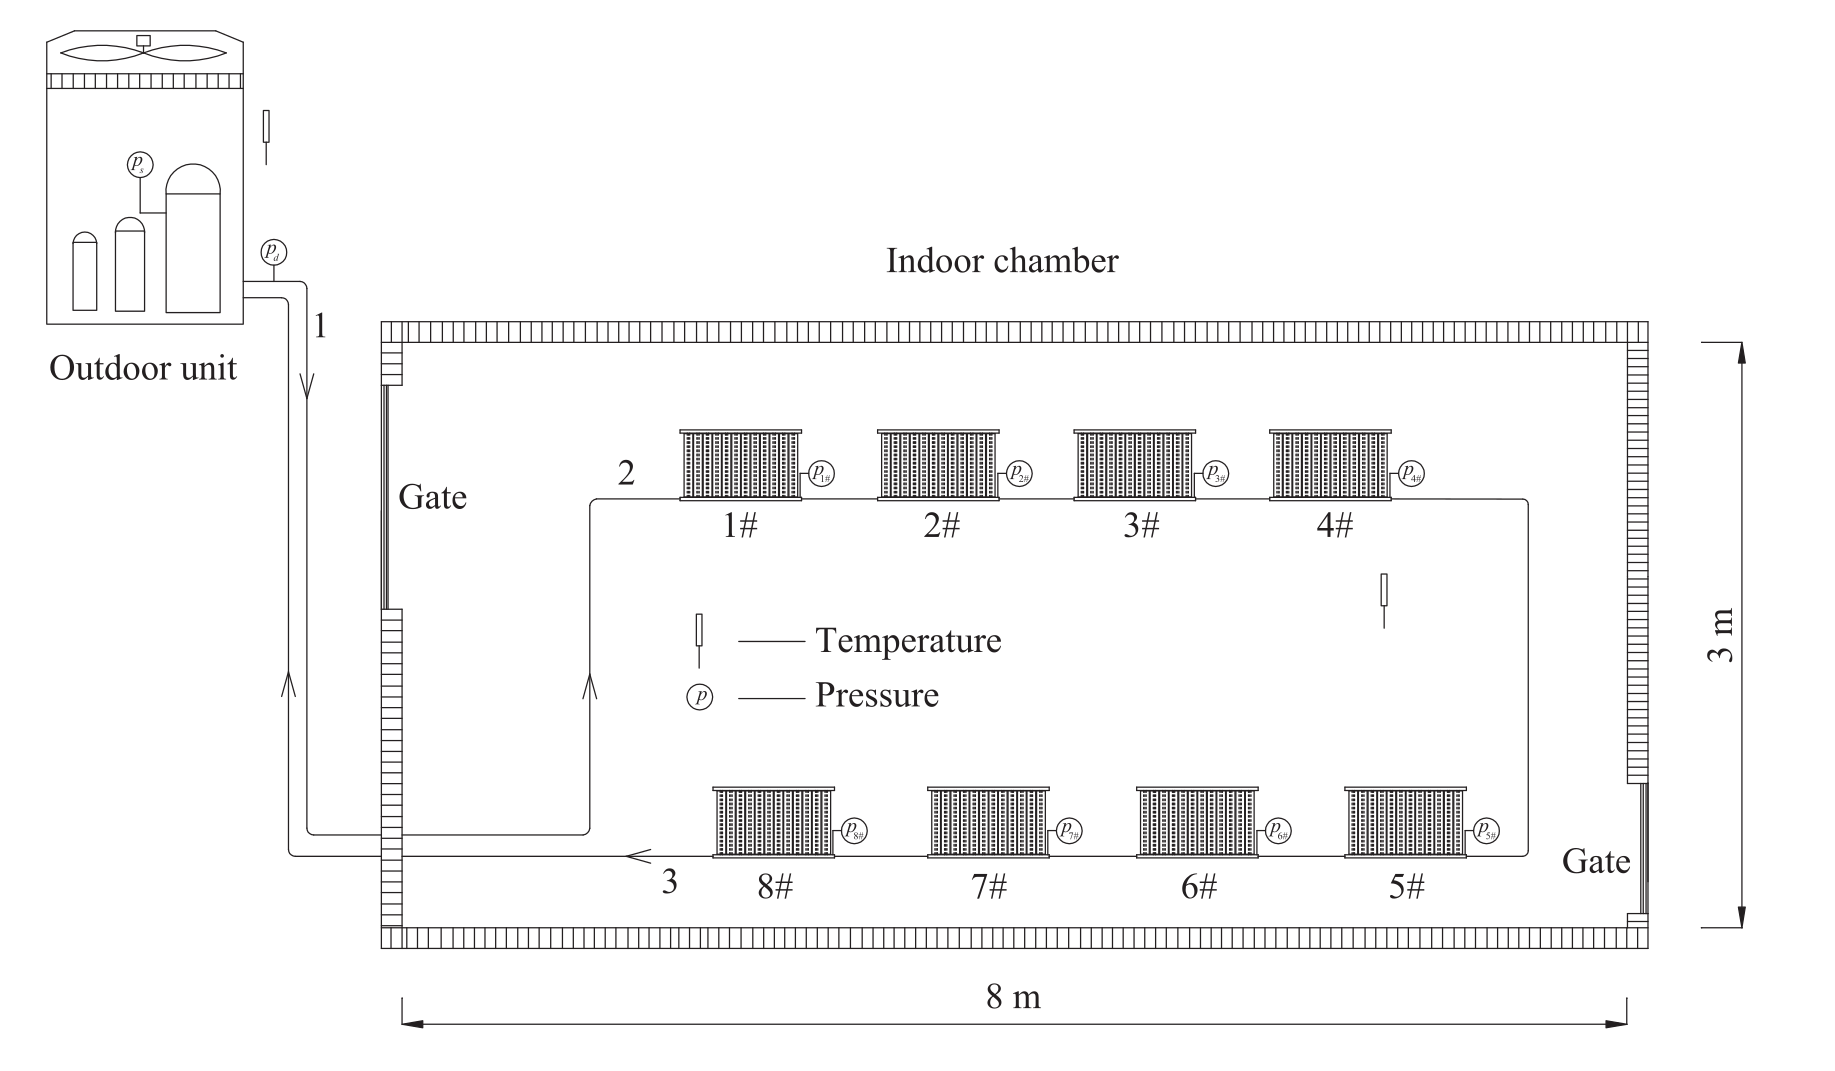
\includegraphics[width=0.7\textwidth]{picture/picture_5}
	\caption{原生测试系统示意图}
	\label{F:5}
\end{figure}

\begin{figure}[h]
\centering  %图片全局居中
\subfigure[外部单元]{
\label{F:6a}
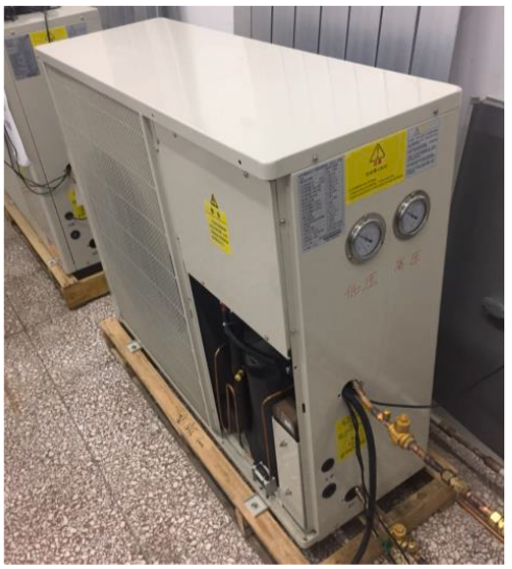
\includegraphics[width=0.3\textwidth]{picture/picture_6_a}}
\subfigure[内部单元]{
\label{F:6b}
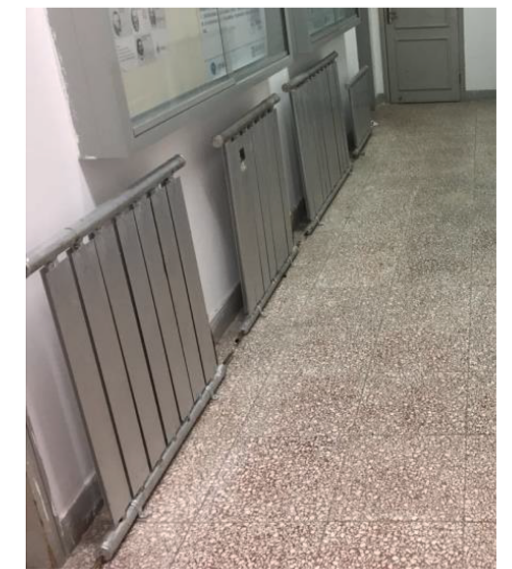
\includegraphics[width=0.3\textwidth]{picture/picture_6_b}}
\caption{ASHPMP 系统照片}
\label{F:6}
\end{figure}

\begin{table}[ht]
	\centering
	\caption{ASHPMP 系统特性}
	\begin{tabular}{@{}ll@{}}
		\toprule
		参数 	& 值/细节 \\ \midrule
		压缩机  & \\
		~压缩机类型  & 滚动活塞 \\
		~输入功率$\unit{\kW} $  & 0 \textasciitilde $\qty{3}{\kW} $ \\
		~制冷剂  & R410A \\
		EEV  & \\
		~模型  & CAREL $E^2 V$ \\
		室外热交换  & \\
		~类型  & 铜管/铝鳍片\\
		~额定容量 $\unit{\kW}$  & 8 \\
		~数量  & 1 \\
		室内交换器  & \\
		~类型  & HPR\\
		~额定容量 $\unit{\kW}$  & 1.2 \\
		~数量  & 8 \\
		~制冷剂  & R134a \\ \bottomrule
	\end{tabular}
	\label{T:2}
\end{table}

\begin{table}[ht]
	\centering
	\caption{实验参数的不确定性}
	\begin{tabular}{@{}llll@{}}
		\toprule
		传感器 & 精确度 & 全量程 & 模型 \\ \midrule
		温度传感器 & $\pm\qty{0.15}{\degreeCelsius} $ & - & Pt100 \\
		压力传感器 & $\pm 0.5\%$ 全量程 & $\qty{4.0}{\MPa} $ & Huba \\
		流量计 & $\pm 0.2\%$ 全量程 & $\qty{250}{\g/\s} $ & Shouke \\
		电力采集单元 & $\pm 0.5\%$ 全量程 & $\qty{10}{\kW} $ & DZFC-1 \\
		数据采集器 & $\pm 0.2\%$ 全量程 & - & HP34972A \\
		加热能力 & $2.9\%$ & & \\
		热 COP & $3.9\%$ & & \\ \bottomrule
	\end{tabular}
	\label{T:3}
\end{table}


\section{试验结果与讨论}
在冬季,北京的最低温度可达$\qty{-20}{\degreeCelsius} $。热管表面的温度分布、热管表面温度随压缩机启动和停止的波动热管表面温度随压缩机启动和停止的波动。这些数值将影响供暖舒适度和热交换面积的利用率。热交换面积的利用率。此外,热泵的冷凝温度与热管内部饱和温度之间的差值也被监测。此外,还对热泵冷凝温度与热管内部饱和温度之差进行了监测,这也是影响系统供热舒适度的一个重要参数。这是影响系统供暖效率的一个重要参数。


\begin{figure}[htbp]
	\centering
	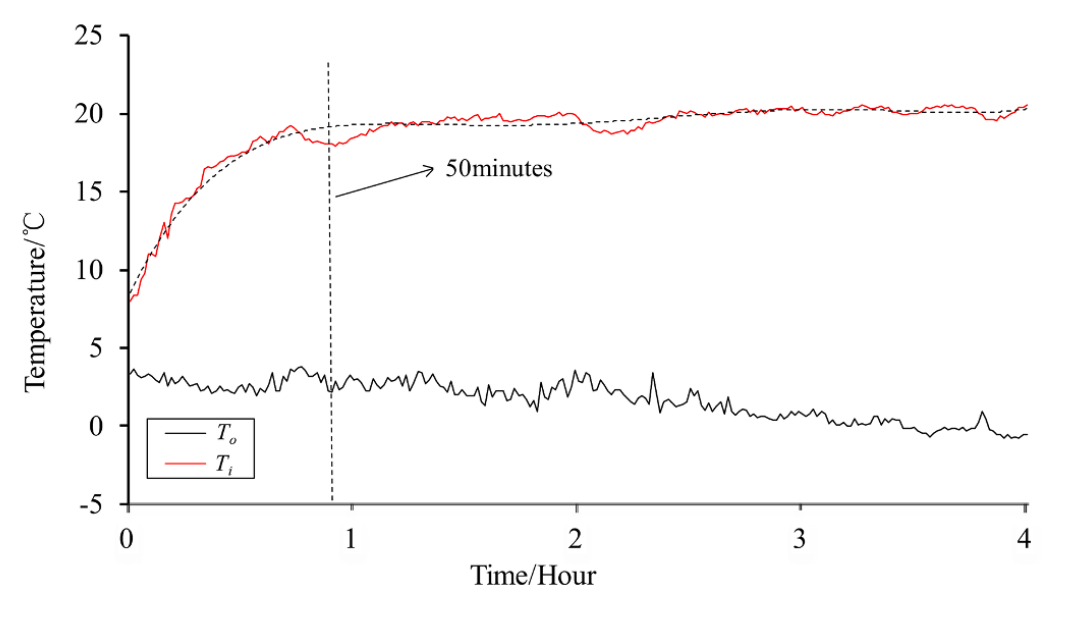
\includegraphics[width=0.7\textwidth]{picture/picture_7}
	\caption{启动时内外温度的变化}
	\label{F:7}
\end{figure}

\subsection{开始处理}
图~\ref{F:7} 显示了系统启动时室内外温度的变化。室外温度为$\qty{-1.5}{\degreeCelsius} $~\textasciitilde~$\qty{3.2}{\degreeCelsius} $,初始室内温度为$\qty{8.2}{\degreeCelsius} $。室内温度开始缓慢上升,温度上升呈现先快后慢的趋势。先快后慢的趋势。约 50 分钟后,室内温度
温度达到最高值约$\qty{20}{\degreeCelsius} $,然后,室内温度基本维持在约 
$\qty{20}{\degreeCelsius} \pm \qty{2}{\degreeCelsius} $左右。

\subsection{温度分布}
图~\ref{F:8} 和图~\ref{F:9} 显示了室内温度达到设定值约一小时后的温度变化情况。HPR 表面最高温度为$\qty{40}{\degreeCelsius} $ \textasciitilde~$\qty{50}{\degreeCelsius} $ (运行时),最小温度$\qty{27}{\degreeCelsius} $ \textasciitilde~$\qty{29}{\degreeCelsius} $(停止时)。

除第一个 HPR 外,其他 HPR 的表面温度大致相同。例如,HPR \#1的表面温度为$\qty{40}{\degreeCelsius} $,而最后 HPR \#8 的表面温度为$\qty{37}{\degreeCelsius} $。室外温度$T_o$为$\qty{5}{\degreeCelsius} $。第一个 HPR \#1 的表面温度比其他 HPR 高出约$\qty{3}{\degreeCelsius} $。

图~\ref{F:8} 和图~\ref{F:9} 还显示了第一个 HPR \#1 和其他 HPR 表面温度的差异。室外温度越低,表面温差越大。HPR \#1 的表面温度比其他 HPR 高约$\qty{8}{\degreeCelsius} $。原因是当室外温度较低时,压缩机的排气温度较高,而当室外温度较高时,压缩机的排气温度较低。温度较高时,第一个 HPR 将从压缩机接收温度最高的制冷剂。因此,第一个 HPR 与其他 HPR 之间的表面温差会增大。

\begin{figure}[htbp]
	\centering
	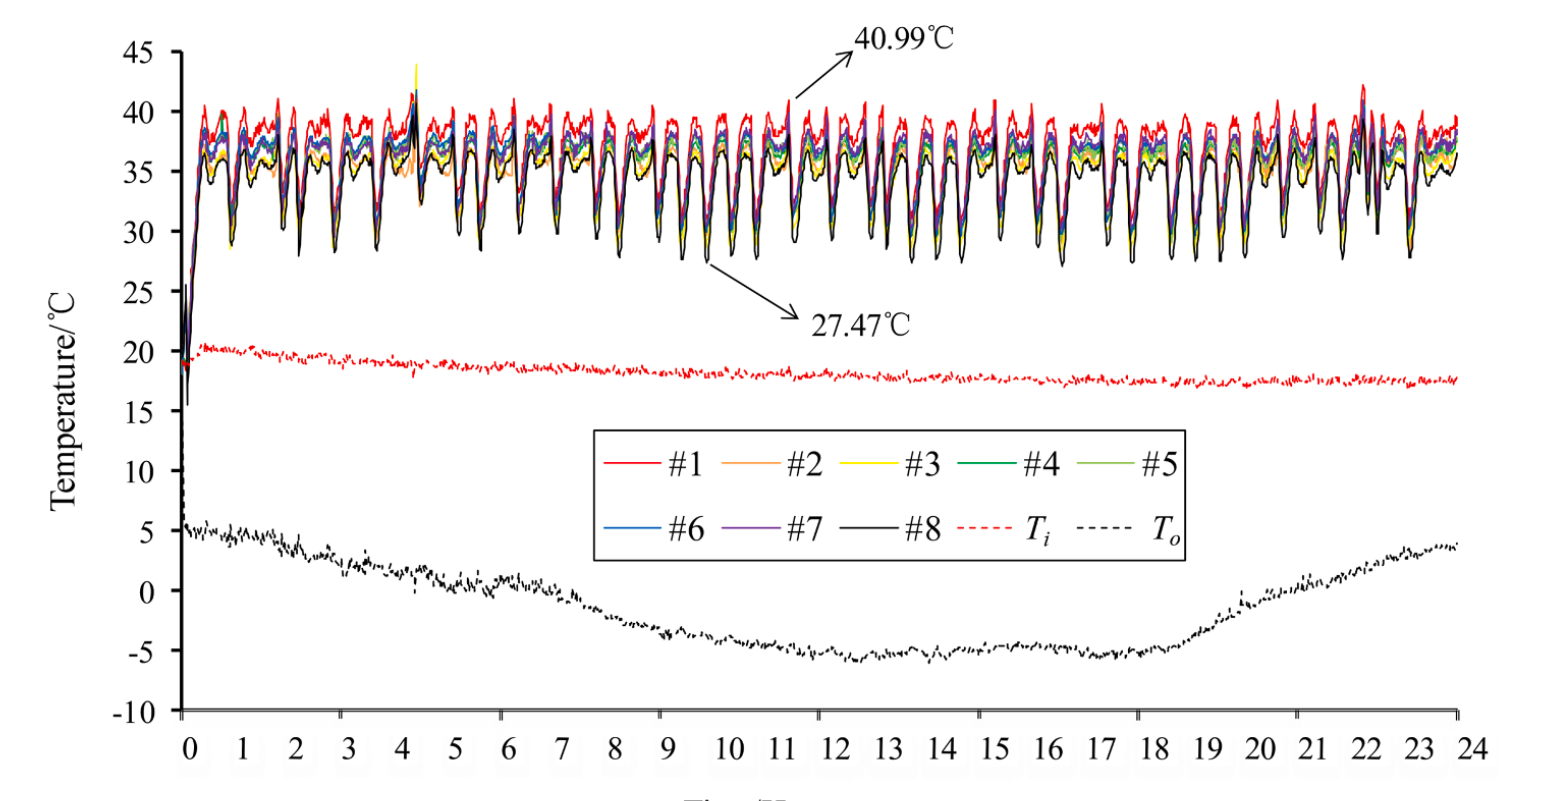
\includegraphics[width=0.7\textwidth]{picture/picture_8}
	\caption{HPRs 的温度特性 $T_o = \qty{-5}{\degreeCelsius}$ \textasciitilde $\qty{5}{\degreeCelsius}$}
	\label{F:8}
\end{figure}

\begin{figure}[htbp]
	\centering
	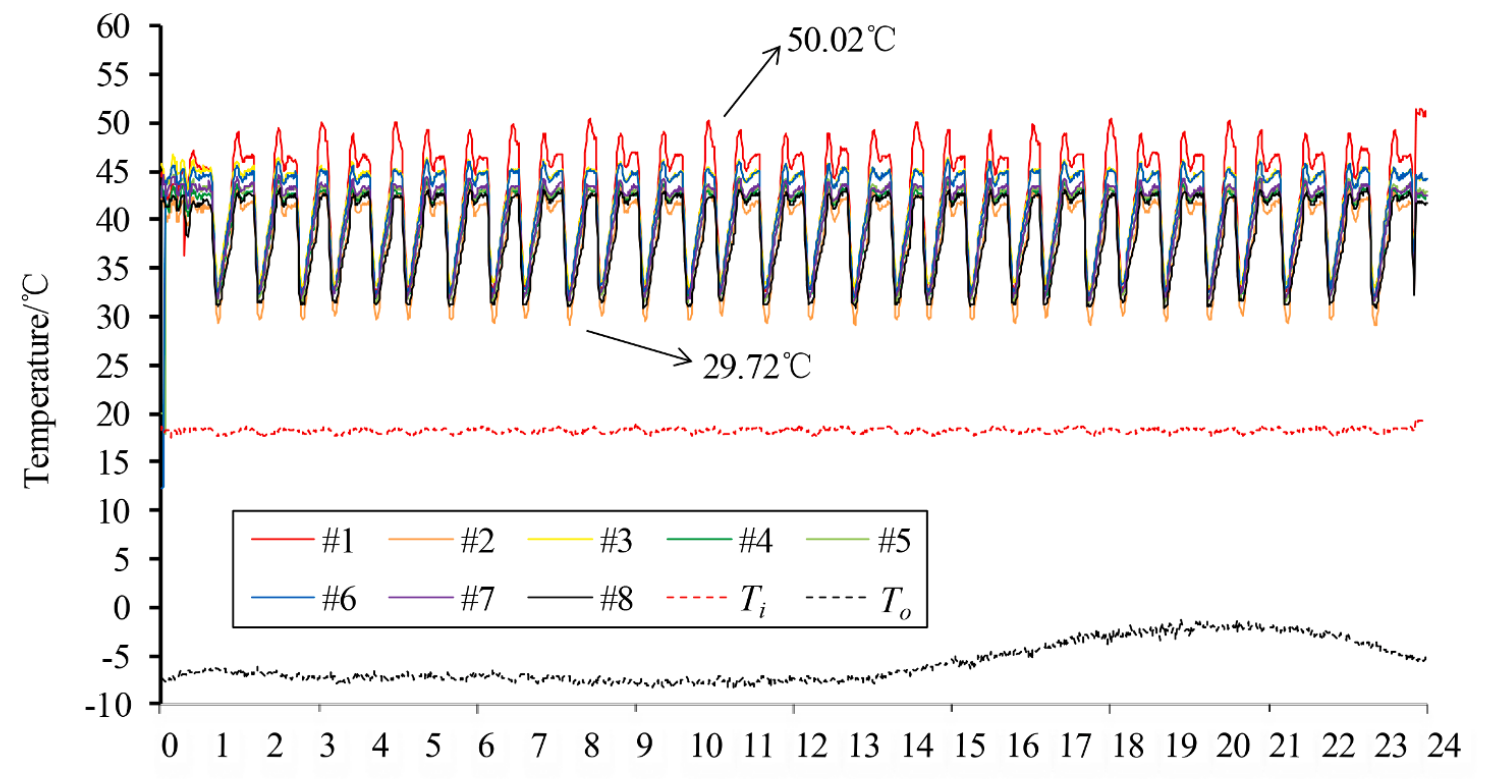
\includegraphics[width=0.7\textwidth]{picture/picture_9}
\caption{HPRs 的温度特性 $T_o = \qty{-7}{\degreeCelsius}$ \textasciitilde $\qty{-4}{\degreeCelsius}$}
	\label{F:9}
\end{figure}

\subsection{压力变化}
图~\ref{F:10} 显示了 8 组 HPR 在运行过程中压缩机吸气压力、排气压力和内部压力的变化情况。所有压力参数都随着启动过程发生周期性变化,时间段约为 35 分钟。随着系统的运行,热管内部压力的变化趋势与热泵的冷凝压力一致。例如,当运行 40 分钟时,HPRs 的压力达到约$\qty{1.12}{\MPa} $,压缩机的排气压力也上升到约 $\qty{2.72}{\MPa} $,压缩机吸气压力保持在约$\qty{0.42}{\MPa} $。8 组 HPR 的压力各不相同,其值呈现出以下特征 值显示出以下特征:
 \[
 	p(\#1) > p(\#2) \approx p(\#3) \approx p(\#4) \approx p(\#5) \approx p(\#6) \approx p(\#7) > p(\#8)
 \]

\begin{figure}[htbp]
	\centering
	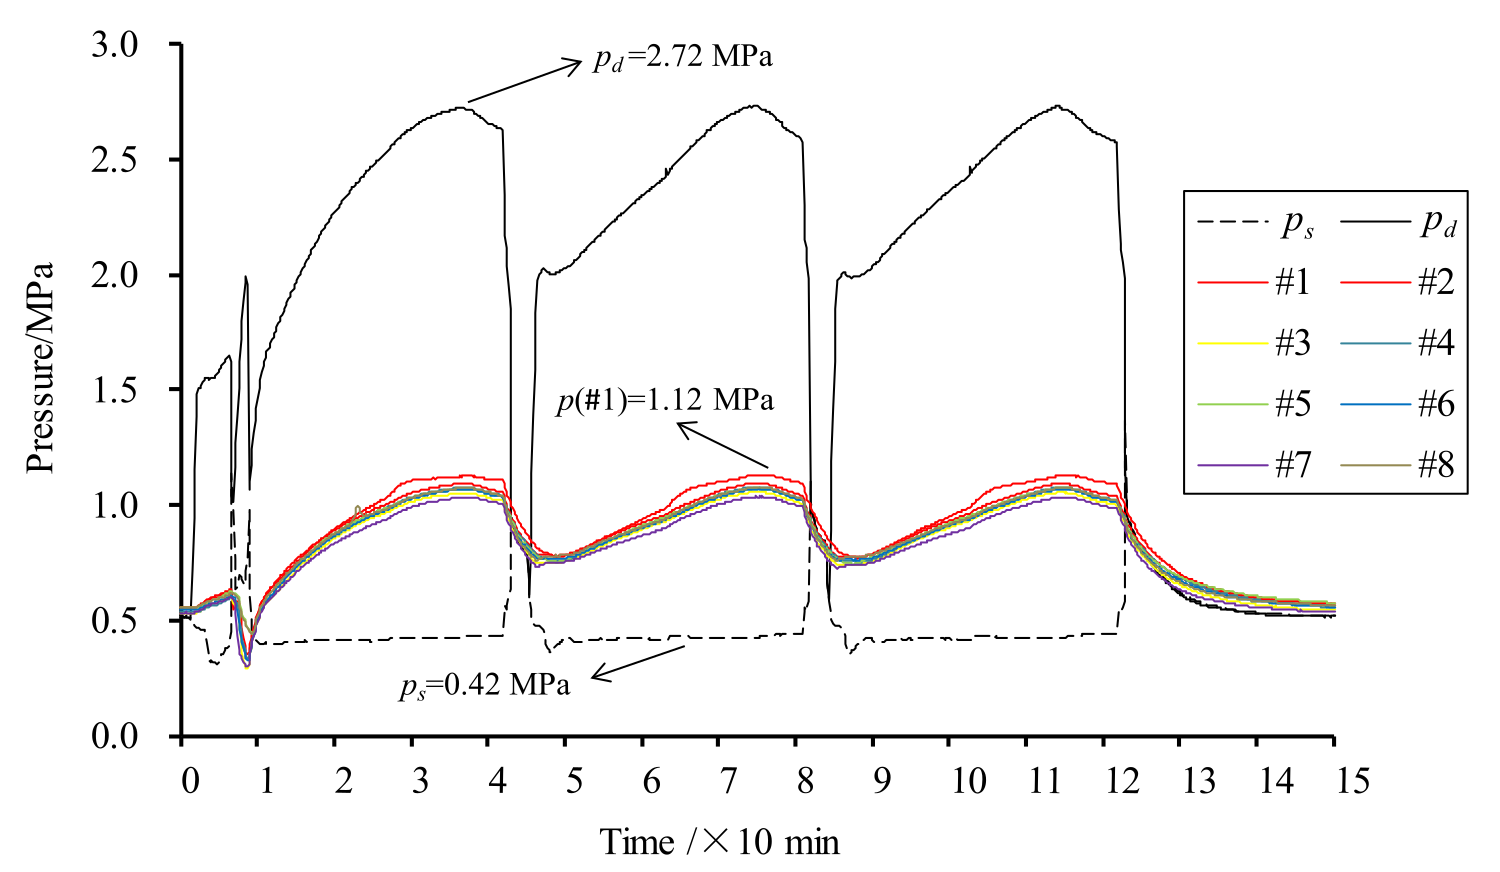
\includegraphics[width=0.7\textwidth]{picture/picture_10}
	\caption{ASHPMP 系统的吸气、排气和内部压力随时间的变化}
	\label{F:10}
\end{figure}

原因可能是:压缩机的高温蒸汽首先进入 HPR \#1,导致其内部压力最高。热泵的工作介质在 \#2、\#3、\#4 $\dots$和\#7 的散热器中发生饱和相变,因此因此 2 号至 7 号 HPR 的内压是一致的。8 号 HPR 中的8 号 HPR 中的工作介质均为液体,具有一定程度的过冷度,因此其内部压力与 2 号至 7 号 HPR 相一致。因此其内部温度是所有热管加热器中最低的。

表~\ref{T:4} 汇总了 8 组 HPR 末端的内部压力和热泵的冷凝压力。从表~\ref{T:4} 中可以看出,热泵的冷凝温度与热管散热器中的饱和温度之差仅为。在$\qty{0.7}{\degreeCelsius} $~\textasciitilde~$\qty{1.8}{\degreeCelsius}$(\#1 和 \#8 除外)。HPR \#1 内部的压力最高,因为高温蒸汽首先进入 HPR \#1; HRP \#8 的压力最低,因为热泵的工作流体已完全凝结为液体。

\begin{table}[ht]
\centering
\caption{$t_{k-heat pump}$ 和 $t_{k-heat pipe}$ 测试结果}
\begin{tabular}{@{}lllllllll@{}}
\toprule
\multirow{2}*{$t_{k-heat pump}/\unit{\degreeCelsius}$} & \multicolumn{8}{l}{$t_{k-heat pipe}/\unit{\degreeCelsius} $} \\
\cmidrule{2-9} & \#1 & \#2 & \#3 & \#4 & \#5 & \#6 & \#7 & \#8
\\ \midrule
39.5 & 42.6 & 38.7 & 38.5 & 38.3 & 38.7 & 38.8 & 38.6 & 37.5 \\
42.5 & 46.5 & 41.7 & 41.5 & 41.8 & 41.3 & 41.6 & 41.2 & 40.5 \\
44.9 & 50.2 & 43.9 & 43.3 & 43.2 & 43.7 & 43.1 & 43.1 & 41.5 \\ \bottomrule
\end{tabular}
\label{T:4}
\end{table}

\subsection{结霜和除霜过程中的工作特性}
图~\ref{F:11} 到 \ref{F:13} 显示了除霜过程中 HPR 表面温度的变化。与传统的空气源热泵一样,ASHPMP 系统的室内机在除霜过程中温度也会下降。首先,必须确保空气中的水蒸气不会在室内机表面凝结成水;其次,室内机的表面温度不能低到让人感觉不舒服,而且除霜过程的时间不能太长。因此,有必要在化霜 + 除霜过程中监控室内机的表面温度。选择了 \#1、\#4 号和 \#8 热管散热器。观察高度方向上的三个温度观察高度方向上的三个温度点,分别是顶部、中心和底部。和底部。从图~\ref{F:11} 到 \ref{F:13} 中可以看出,随着化霜的开始,室内空调的表面温度逐渐升高。所有 HPR 的表面温度都迅速下降。

在除霜过程中,HPR 的表面温度大大降低。热泵的冷凝器变成了蒸发器,它吸收了热管内工作流体的热量和热管壁的显热。热管内工作流体的热量包括液体的显热和蒸汽冷凝成液体的潜热。蒸发器的吸热量是否能满足除霜所需的热量,取决于热管中工作介质的充注量以及工作介质的显热和潜热之和。工作流体在 HPR 中的显热和潜热之和。

解冻过程停止后,系统重新开始加热,HPR 表面温度继续升高至正常工作状态,整个过程持续了约 20 分钟。在整个工作过程中,除霜和融霜时间约为 80 分钟。在除霜过程中,HPRs 底部表面温度下降最明显,约为$\qty{30}{\degreeCelsius} $。主要原因是解冻时采用了逆循环解冻,实际上是一个制冷过程,因此越靠近底部,就越靠近冷却盘管。与 HBR \#1、\#4和 \#8 相比,发现 HPR 
\#8 的表面温度下降幅度最大,而 HPR \#1 的表面温度下降幅度最小。主要原因是 系统从加热模式切换到制冷模式,制冷剂反向循环,低温制冷剂首先进入 \#8,然后进入 \#4,最后进入 \#1。

\begin{figure}[htbp]
	\centering
	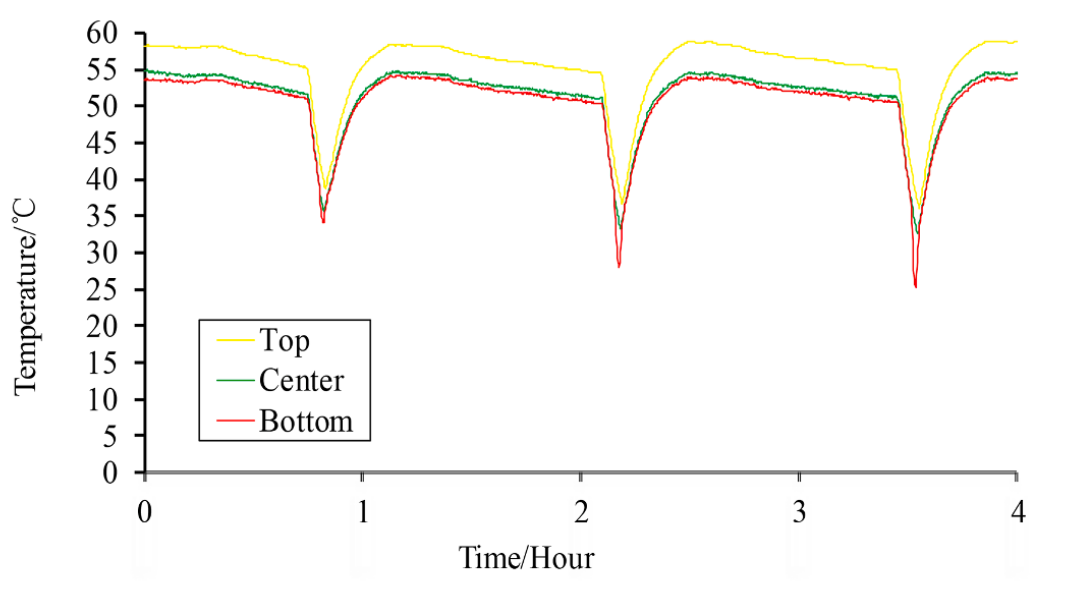
\includegraphics[width=0.7\textwidth]{picture/picture_11}
	\caption{表面温度分布结霜和解霜过程 (HPR \#1)}
	\label{F:11}
\end{figure}

\begin{figure}[htbp]
	\centering
	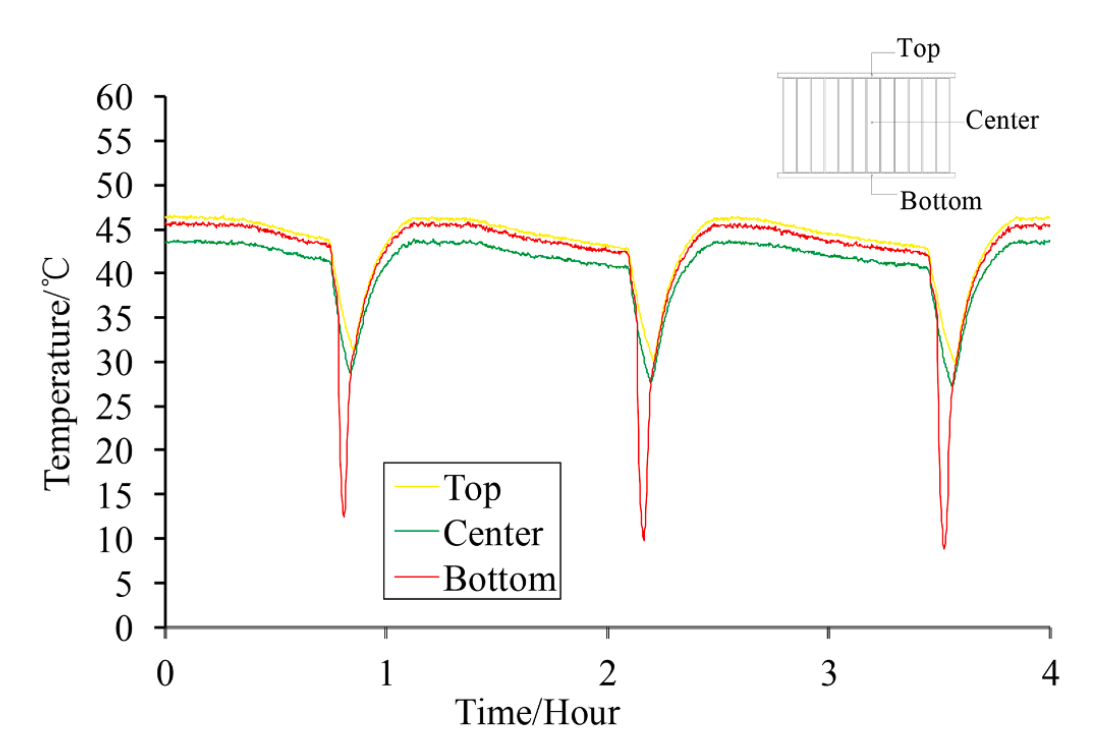
\includegraphics[width=0.7\textwidth]{picture/picture_12}
	\caption{表面温度分布结霜和解霜过程 (HPR \#4)}
	\label{F:12}
\end{figure}

\begin{figure}[htbp]
	\centering
	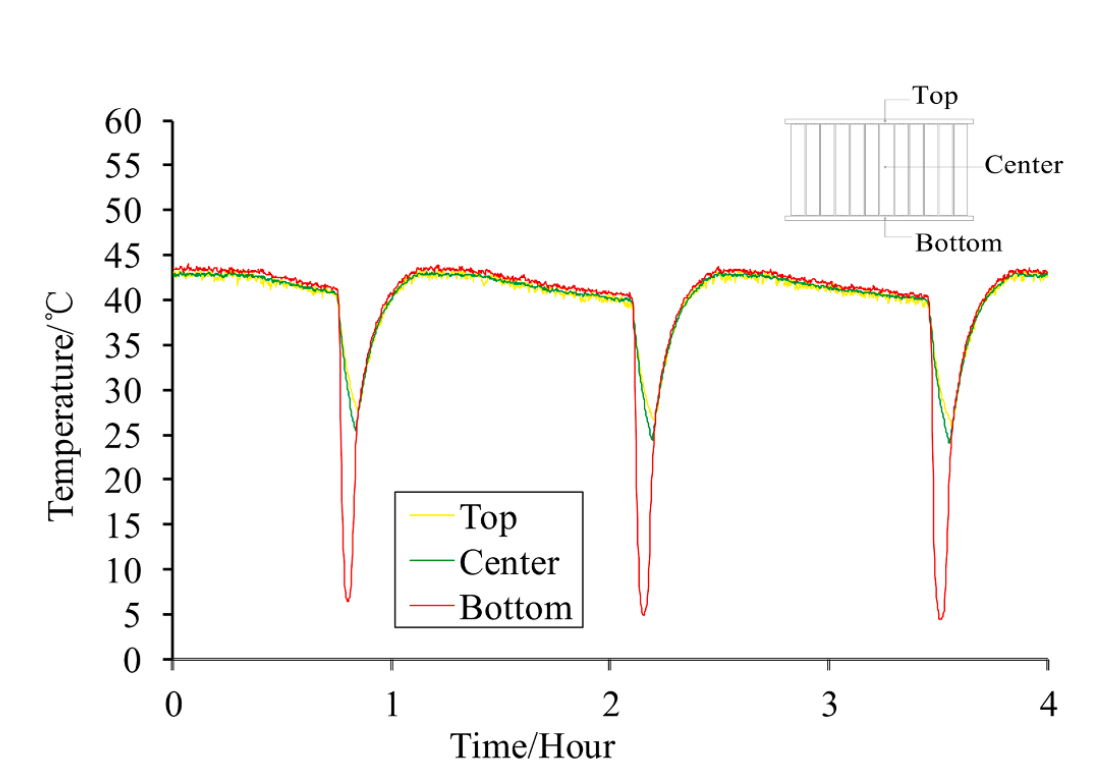
\includegraphics[width=0.7\textwidth]{picture/picture_13}
	\caption{表面温度分布结霜和解霜过程 (HPR \#8)}
	\label{F:13}
\end{figure}

\begin{figure}[htbp]
	\centering
	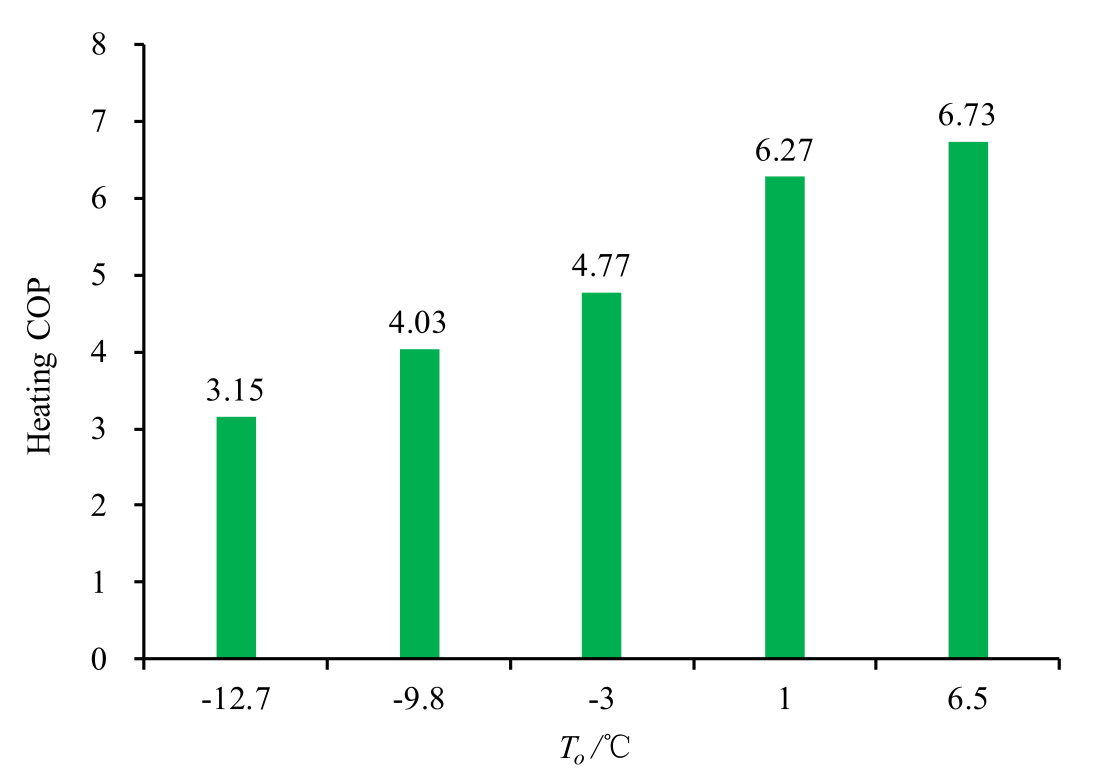
\includegraphics[width=0.7\textwidth]{picture/picture_14}
	\caption{在室外不同温度下的供热 COP}
	\label{F:14}
\end{figure}

\subsection{ASHPMP 系统的供热性能}
不同室外温度下加热 COP 的变化如图~\ref{F:14} 所示。室内温度为$\qty{20}{\degreeCelsius} $。从图~\ref{F:14} 中可以看出,在室外温度为$\qty{-12.7}{\degreeCelsius}$ 时,制热 COP 仍可达到 3.15,而在室外温度为$\qty{6.5}{\degreeCelsius} $ 时,制热 COP 可达到 6.73。

\begin{figure}[h]
\centering  %图片全局居中
\subfigure[外部单元]{
\label{F:15a}
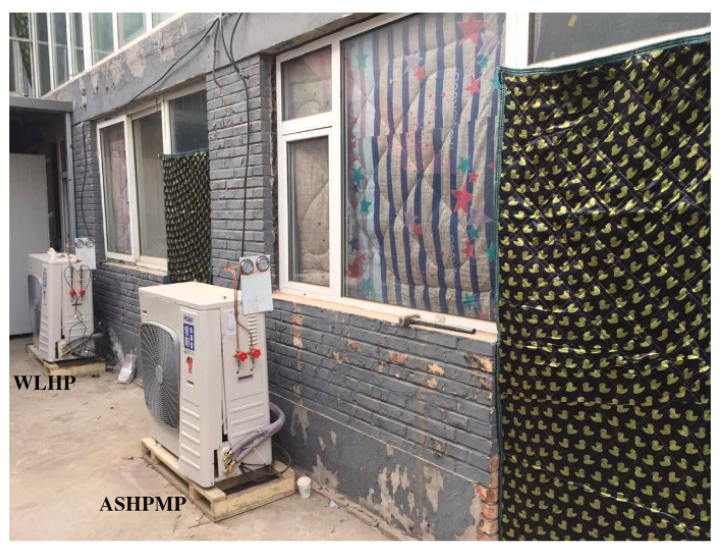
\includegraphics[width=0.3\textwidth]{picture/picture_15_a}}
\subfigure[内部单元]{
\label{F:15b}
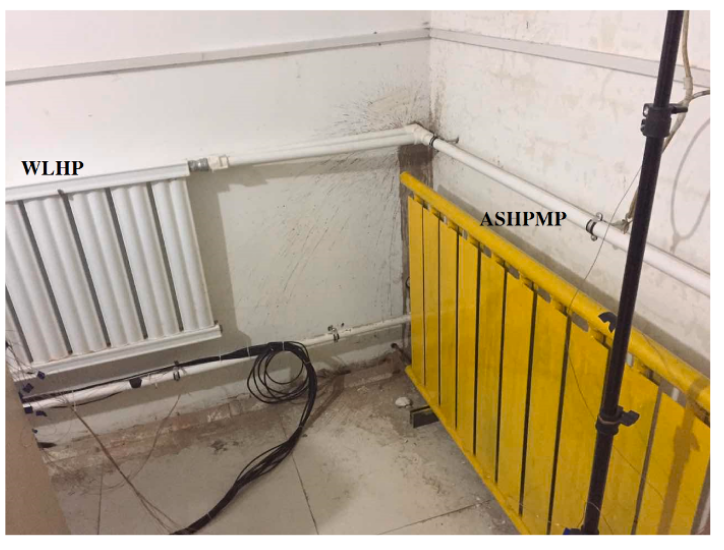
\includegraphics[width=0.3\textwidth]{picture/picture_15_b}}
\caption{加热原型}
\label{F:15}
\end{figure}
\subsection{与水环热泵比较}

为了进一步比较 ASHPMP 系统与水环热泵 (WLHP) 系统的性能,在中国河北省的同一房间内安装了两套系统进行供暖试验,总面积约为$\qty{60}{\m^2}$,共有四个房间。室外机的型号和尺寸相同,室内散热器的总面积和数量也相同。图是实际供暖样机的照片,图显示了两个系统的室外机。在图中,白色单元是水循环系统的室内单元,黄色单元是水循环系统的室外单元。在供暖季节,不同的系统每隔一天轮流运行。在供暖季节,不同的系统每隔一天轮流运行。

图~\ref{F:16} 显示了 ASHPMP 系统和 WLHP 系统在实际运行时吸气压力和排气压力的比较结果。可以看出,在室外温度相同的情况下,两个系统的吸气压力差基本相同,但在排气压力方面,ASHPMP 系统比 WLHP 系统高出约$\qty{0.2}{\MPa} $。主要原因是 ASHPMP 系统存在相变传热,热阻大大降低。WLHP 系统使用水作为中间传热介质 传热温差较大。

表~\ref{T:5} 显示了 ASHPMP 与 WLHP 的制热 COP 比较结果。在室内外温度相同的情况下,ASHPMP 系统的制热 COP 比 WLHP 系统高 36\%~\textasciitilde~72 \%。

值得注意的是,经过 3 个月的测试,ASHPMP 系统具有良好的物理稳定性。即使在结霜/除霜条件下,它仍能为房间提供正常的供暖。在运行成本方面,ASHPMP 系统和 WLHP 系统的室内温度均保持在$\qty{17.4}{\degreeCelsius} $至$\qty{20.4}{\degreeCelsius} $之间。操作时间为$\qty{24}{\hour} $,比较结果如表~\ref{T:6} 所示。结果表明,在室外温度和室内温度大致相同、运行时间相同的条件下,ASHPMP 系统的耗电量为$\qty{31.9}{\kWh} $,WLHP 系统的耗电量为$\qty{59.3}{\kWh} $。ASHPMP 系统可节约 节能约 46.2\%。

\begin{figure}[htbp]
	\centering
	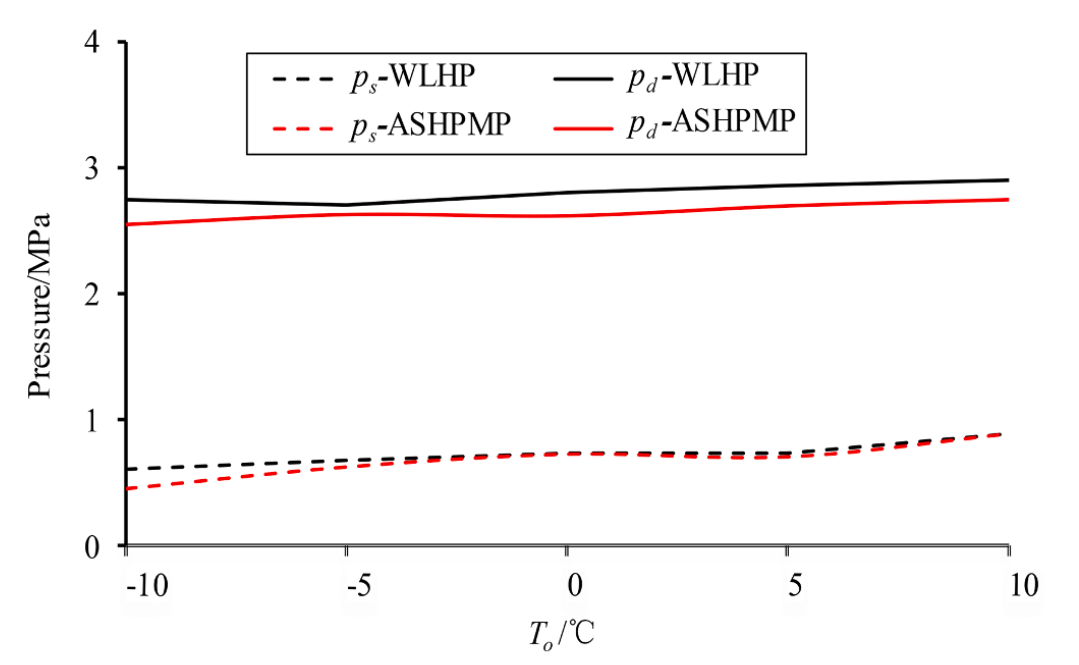
\includegraphics[width=0.7\textwidth]{picture/picture_16}
	\caption{ASHPMP 系统与 WLHP 系统吸气压力和排气压力的比较系统和 WLHP 系统的吸气压力和排气压力的比较}
	\label{F:16}
\end{figure}

\begin{table}[ht]
\centering
\caption{供热 COP 比较}
\begin{tabular}{@{}llll@{}}
\toprule
室内温度 $\unit{\degreeCelsius} $                        & 室外温度$\unit{\degreeCelsius} $                     & WLHP & ASHPMP \\ \midrule
\multirow{3}{*}{18 $\sim$20} & $-12 \pm 1$ & 2.3  & 3.15   \\
                             & $-3 \pm 1$  & 3.2  & 4.77   \\
                             & 6.5       & 3.9  & 6.73   \\ \bottomrule
\end{tabular}
\label{T:5}
\end{table}

\begin{table}[ht]
\centering
\caption{电能消耗结果}
\begin{tabular}{@{}lllll@{}}
\toprule
时间 & 系统 & 室外温度 & 室内温度 & 电能消耗 \\ \midrule
From 07:00,1/2/2019 到 07:00,2/2/2019&  WLHP & -6.5 \textasciitilde $\qty{3.8}{\degreeCelsius}$ & 17.9 \textasciitilde $\qty{19.2}{\degreeCelsius}$  & $\qty{59.3}{\kWh}$  \\
From 06:00,11/2/2019 到 06:00,12/2/2019& ASHPMP & -5.6 \textasciitilde $\qty{4.8}{\degreeCelsius}$ & 17.4 \textasciitilde $\qty{20.4}{\degreeCelsius}$  & $\qty{31.9}{\kWh} $ \\ \bottomrule
\end{tabular}
\label{T:6}
\end{table}

\subsection{结果与推测}
提出了一种采用多组热管散热器的空气源热泵 (ASHPMP) 用于家庭供暖。在 ASHPMP 系统中,冷凝器和热管耦合在一起,形成一种新型的径向末端。研究人员开发了一个共有八个末端的实验装置,并在环境控制室进行了测试。压力、温度 以及热泵和热管的其他参数进行了研究。实验。还探讨了结霜/除霜条件下系统加热性能的变化。结霜/除霜条件下系统加热性能的变化。ASHPMP 系统的工作性能 与水环热泵系统的工作性能进行了比较。本研究还得出了以下结论:
\begin{enumerate}
	\item 在 ASHPMP 系统的初始处理阶段,内室温度在 50 分钟内达到最大值$\qty{20}{\degreeCelsius} $,并在之后维持。
	\item 除第一个热管散热器外,其他热管散热器的表面温度大致相同。其他热管散热器的表面温度基本一致。第一个散热器的表面温度比其他散热器高出约3 \textasciitilde~$\qty{8}{\degreeCelsius} $。高于其他散热器。
	\item 热泵冷凝温度与热管饱和温度的平均差仅为 热泵的冷凝温度与热管饱和温度的平均差仅为$\qty{0.7}{\degreeCelsius}$ \textasciitilde~$\qty{1.8}{\degreeCelsius} $,这使得系统具有较高的能效。
	\item 在解冻过程中,底部温度下降最明显,约为$\qty{30}{\degreeCelsius} $,而顶部温度下降最少。温度下降最少。\#8 散热器的表面温度下降幅度最大,\#1 散热器下降幅度最小。
	\item 在室外温度为$\qty{-12.7}{\degreeCelsius} $ 和$\qty{6.5}{\degreeCelsius} $时,加热 COP 仍可分别达到 3.15 和 6.73。ASHPMP 系统的加热 COP 比 WLHP 系统高出 36\%~\textasciitilde~72\%、 ASHPMP 系统的能耗可节省约 46.2\% 的能源。
\end{enumerate}

在测试室和住宅楼进行的实验结果表明 通过在试验室和住宅楼中进行的实验结果证明 这种新型 ASHPMP 系统在室内供暖方面取得了良好的性能。还有一些问题需要进一步考虑:

首先,新供热系统的研究局限性可能在于设备的频繁启动和停止是一个需要解决的关键问题;其次,应注意如果系统以制冷模式运行,则热管加热端需要进行改造,以具备制冷功能;第三,在串联结构形式下,如何关闭 ASHPMP 系统的一端,是一个重要的实际问题。

\section*{竞争利益声明}
作者声明,他们没有已知的竞争性经济利益或个人关系影响本文所报告的工作。

\section*{致谢}
本项目由河北省教育厅科技项目(批准号:ZD2022116)、河北省邮政局科技项目
河北省教育厅科技项目(批准号:ZD2022116)、河北省 "冷热源工程 "研究生示范 "冷热源工程 "建设项目(批准号:KCJSX2021084)、河北省研究生 "冷热源工程 "示范课大中学生科技创新能力培养专项(批准号:KCJSX2021084)。

\end{document}
